%# -*- coding: utf-8-unix -*-
%%==================================================
%% chapter03.tex for SJTU Master Thesis
%% software requirement specification
%%==================================================
%\bibliographystyle{sjtu2}%[此处用于每章都生产参考文献]

\chapter{相似轨迹查询系统设计与实现}
\label{chap:system requirement specification}

\section{本章序言}
\label{sec:introduction}
随着相似轨迹查询这以在科研领域和工业应用中的不断发展,开发相似轨迹查询系统为用户在搜索相似轨迹中提供更方便更可视化的结果。为了明确关于相似轨迹查询系统的设计需求、应用领域与系统功能,在本章节中,本文首先对相似轨迹查询系统的设计与实现作细节说明和具体描述。我们对本章节的目的以及之后说明中会涉及到的名词概念进行解释,以便于之后章节的拓展。该系统是主要以Python进行后端数据处理,系统运行于以Python为基础的Flask Web内部依赖Werkzeurg的工作集服务器。用户只需要通过进行简单操作便可以实现个性化的相似轨迹查询操作,并了解本系统软件的基本工作原理。

\subsection{系统设计编写背景}
\label{subsec:target}
待开发的系统为相似轨迹查询系统。本章节设计概要可作为系统设计人员、系统测试人员、系统使用用户的参考资料与文档。设计实现服务对象为需要进行相似轨迹查询的互联网用户。

\subsection{系统设计编写原则}
\label{subsec:principle}
\begin{itemize}
	\item 准确性:本章节所描述的针对系统的需求,设计系统的功能与行为与目标软件系统产品实现期望相符。
	\item 完整性:包括全部有实际应用意义的系统需求,在功能、性能和设计方面均满足所需的需求。依照<系统软件设计规范说明书>\cite{tuw2002software}的要求,将描述系统需求所需的流程图和名词定义给出完整描述。
	\item 易读性:本章节内容通过简要文字,辅以插图和图标,让读者对象能够清楚了解系统设计中的需求内容。
	\item 可验证性:对于本章节中所编写的系统需求分析与设计内容,读者可通过实际系统进行功能、性能和设计方面上的检查以校对是否与编写内容一致。
\end{itemize}

\subsection{系统名词定义}
\label{subsec:definitions}
表\ref{tab-system definitions}所示。
\begin{table}[!htpb]
  	\centering
		\begin{tabular}{ |p{3cm}||p{9cm}|  }
		\hline
		符号标记 & 符号注释 \\
		\hline
		用户 & 使用相似轨迹查询系统进行轨迹查询人员 \\
		\hline
		管理员 & 相似轨迹查询系统管理员,负责运行权限和控制系统 \\
		\hline
		轨迹数据 & 移动物体上空间上按时间顺序的移动数据记录 \\
		\hline
		GPS & 全球定位系统 \\
		%\hline
		%DESC & 描述 \\
		%\hline
		%DEP & 依赖 \\
		\hline
		\end{tabular}
	\bicaption[tab-system definitions]{相似轨迹查询系统涉及名词定义}{相似轨迹查询系统涉及名词定义}{Table}{A list of definitions and explanations in the system of searching similar trajectories}
\end{table}

\subsection{用户类与特点}
\label{subsec:user characteristics}
相似轨迹查询系统的使用者主要分为轨迹查询用户和管理用户。

对于轨迹查询用户而言,我们通过是否具有在系统中存储这历史轨迹数据分为登录用户和一般用户。一般用户是系统的流动用户,在系统轨迹数据库中不具备历史轨迹。一般用户只能通过向系统输入一组轨迹查询点集以完成相似轨迹查询功能。登录用户可以根据账户信息和密码登录相似轨迹查询系统,使用已有的历史轨迹数据或是自定义的一组轨迹点集实现相似轨迹查询功能。

相似轨迹查询系统中的管理员主要负责登录用户的权限管理和对历史数据的修改处理操作。管理员对于相似轨迹查询系统中违反查询和使用规范的用户可以修改其登录权限以阻止其进一步违规操作。管理员还可以对历史轨迹进行增加、修改和删除操作,以保证系统数据库的实时性和准确性。

\subsection{系统运行环境}
\label{subsec:system environment}

表\ref{tab-system environments}对本系统运行环境进行了描述。
\begin{table}[!htpb]
  	\centering
		\begin{tabular}{ |p{1cm}|p{3.5cm}|p{8.5cm}| }
		\hline
		序号 & 环境需求 & 环境参数 \\
		\hline
		01 & 系统操作系统 & Mac OS 10.11.6  \\
		\hline
		02 & 分布式操作系统 & Ubuntu14.04.1 amd64  \\
		\hline
		03 & 单机PC设备参数 & 处理器 2.6 GHz Intel Core i5且内存大于等于4G\\
		\hline
		04 & 分布式PC设备参数 & 处理器 2.6 GHz Intel Core i5且内存大于等于1G\\
		\hline
		05 & 服务器平台 & Flask0.12/Python2.7.6 \\
		\hline
		\end{tabular}
	\bicaption[tab-system environments]{相似轨迹查询系统运行环境}{相似轨迹查询系统运行环境}{Table}{A list of environment parameters in the system of searching similar trajectories}
\end{table}


\section{系统设计}
\label{sec:overall description}
本文设计的相似轨迹查询系统运行运行于基于Python语言的Flask Web框架,运行过程中需要连接互联网以使用地图接口,系统内部数据为上海私家车数据。系统针对的用户为一般用户和登录用户。一般用户可以目的轨迹点集进行相似轨迹查询,实现路径规划等具体应用,用户在运用过程中需要在地图上点击位置以实现轨迹点击输入;登录用户在一般用户具有功能基础上,用户的历史轨迹在轨迹数据库中有存储,可以实现以一条轨迹为输入的相似轨迹查询,实现拼车或轨迹推荐等具体应用。本系统目前已有依赖于Flask框架和地图接口提供。

\subsection{系统设计分析}
\label{subsec:system build requirement}
将相似轨迹查询系统以Web框架搭建,其最大的好处是给予用户在查询上最大程度的便利。这种便捷主要体现在用户只要连接上互联网,就可以直接通过浏览器访问系统,在线进行相似轨迹的查询。这种网络操作不需要用户在下载系统到终端或者移动端便可以进行实时的相似轨迹查询功能。所以在设计相似轨迹查询这一系统时,主要功能实现均为用户查询而服务,即最重要的一点是完成用户功能部分。

\subsection{系统功能描述}
\label{subsec:product functions}
在相似轨迹查询系统中,一般用户和登录用户都可以使用相似轨迹查询功能。查询结果与用户定义的输入轨迹数据类型(为轨迹点集或一条历史轨迹)、查询的日期、相似轨迹数目阈值和查询是否有序性有关。

在完成登录功能或跳选到直接查询后,用户可以在系统界面中完成查询功任务。相似轨迹查询的主要是通过在地图上以不同颜色和不同粗细的折线端进行表示。在查询结果中,根据与查询输入相似度的相关性,越相似的查询结果轨迹将以越显著的参数表示出来,用户可以一目了然在地图上得出最符合查询的结果的一条或多条轨迹。登录用户可以在地图上点击历史轨迹数据显示系统数据库中存储的某一条与自己相关的历史轨迹。

\subsection{系统设计框架}
\label{subsec:product perspective}
如图\ref{fig:system-architecture}所示相似轨迹查询系统主要由前后端两部分组成。后端部分主要以轨迹预处理、相似轨迹查询和查询请求分析处理为主;前端以部分地图轨迹可视化、查询结果输出、地理位置搜索等部分组成。

\begin{figure}[!htp]
  \centering
  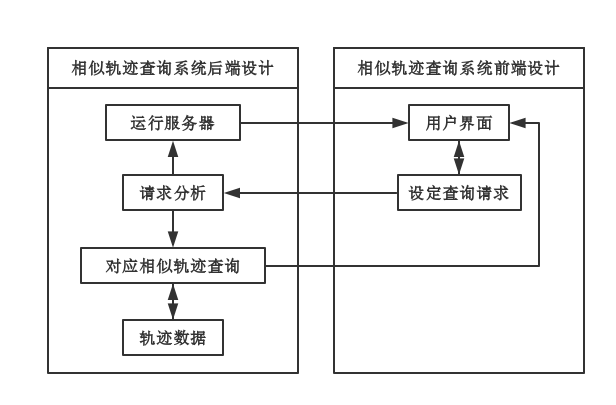
\includegraphics[width=0.8\textwidth]{design/system-architecture.png}
  \bicaption[fig:system-architecture]{相似轨迹查询系统设计框架}{相似轨迹查询系统设计框架}{Fig}{System design architecture}
\end{figure}

针对相似轨迹查询系统的后端处理流程思路主要为,在后台运行服务器代码,接收来自浏览器前端的请求。将请求分析与提前预先设定的资源定位符函数结合,对于数据类型选择是否进行轨迹数据预处理。针对同一的输入轨迹数据点集,进行相似轨迹数据查询功能服务。然后将结果作为请求返回返回给用户。实现一次相似轨迹查询请求过程。与此同时,系统前端主要以实现数据可视化为主,以一个窗口形式将地图数据显示。对于用户感兴趣的地理位置坐标点和历史轨迹数据,可以通过点击地图或历史轨迹数据项目将数据在地图窗口上得以可视化展示。

\subsection{系统处理流程}
图\ref{fig:system-flowchart}展示了相似轨迹查询系统的主要流程。进入相似界面之后,用户可以直接使用系统(即不需要登录)使用系统进行相似轨迹查询,在获取满意的查询结果之后退出系统。同时,如果需要运用登录功能,系统会在登录界面中提醒用户是选择轨迹历史用户登录还是管理员模式登录。对于轨迹历史用户,可以实现相对应的轨迹查询类型并和一般用户一样在得到满意的查询结果之后退出系统。对于管理员而言,他们主要负责对用户权限和轨迹数据处理这一部分工作,在完成管理员工作之后他们也可以按流程退出系统。

\label{subsec:system flow}
\begin{figure}[!htp]
    \centering
    \resizebox{14cm}{!}{
\begin{tikzpicture}[node distance=2cm]

	%\node (input) [startstop] {输入轨迹数据类型判断};
	%\node (input_judge) [decision, below of=input,yshift=-0.5cm,aspect=2.5] {是否为用户指定一组轨迹点集?};
	%\node (ts) [process, right of=input_judge,xshift=5cm] {轨迹简化};
	%\node (iknn) [process, below of=input_judge,yshift=-0.5cm]{增长型k相似轨迹查询};
	%\node (bound_judge) [decision, below of=iknn,yshift=-0.5cm,aspect=2.5]{是否满足相似度上下界条件?};
	%\node (refinement)[process, below of=bound_judge,yshift=-0.5cm]{备选轨迹集筛选};
	%\node (output)[startstop, below of=refinement]{k条最相似轨迹输入};
	

%	\draw [arrow] (input) -- (input_judge);
%	\draw [arrow] (input_judge) -- node[anchor=south]{否}(ts);
%	\draw [arrow] (input_judge) -- node[anchor=west]{是}(iknn);
%	\draw [arrow] (ts) |- (iknn);
%	\draw [arrow] (iknn) -- (bound_judge);
%	\draw [arrow] (bound_judge.west) |- node[anchor=south]{否}(iknn.west);
%	\draw [arrow] (bound_judge.south) -- node[anchor=west]{是}(refinement.north);
%	\draw [arrow] (refinement) -- (output);

	\node (begin) [startstop,font=\bf,fill=green!20] {进入系统界面};
	\node (login_judge) [decision, below of=begin, yshift=-0.5cm, aspect=2.5]{是否需要登录};
	\node (general) [process, right of=login_judge, xshift=3cm]{一般用户};
	\node (login_type_judge) [decision, below of=login_judge, yshift=-0.5cm, aspect=2.5]{是否为管理员};
	\node (history) [process, right of=login_type_judge, xshift=3cm]{登录用户};
	\node (admin) [process, below of=login_type_judge]{管理员操作};
	\node (search) [process, right of=history, xshift=3cm]{相似轨迹查询};
	\node (is_search_good) [decision, below of=search, aspect=2.5]{是否满意查询结果};
	\node (does_admin_finish) [decision, below of=admin, aspect=2.5]{管理员操作是否完成};
	\node (finish) [process, below of=history]{系统处理完成};
	\node (stop) [startstop, below of=finish,font=\bf,fill=green!20]{退出系统界面};
	
	
	
	\draw [arrow](begin.south) -- (login_judge.north);
	\draw [arrow](begin.east) -| node[anchor=south]{直接查询模式}(general.north);
	\draw [arrow](login_judge.east) -- node[anchor=north]{否}(general.west);
	\draw [arrow](login_judge.south) -- node[anchor=west]{是}(login_type_judge.north);
	\draw [arrow](login_type_judge.east) -- node[anchor=north]{否}(history.west);
	\draw [arrow](login_type_judge.south) -- node[anchor=west]{是}(admin.north);
	\draw [arrow](general.east) -| (search.north);
	\draw [arrow](history.east) -- (search.west);
	
	\draw [arrow](search.south) -- (is_search_good.north);
	\draw [arrow](is_search_good.east) |- node[anchor=west]{否}(search.east);
	\draw [arrow](is_search_good.west) -- node[anchor=north]{是}(finish.east);
	
	\draw [arrow](admin.south) -- (does_admin_finish.north);
	\draw [arrow](does_admin_finish.west) |- node[anchor=east]{否}(admin.west);
	\draw [arrow](does_admin_finish.east) |- node[anchor=east]{是}(finish.west);
	
	\draw [arrow](finish.south) -- (stop.north);

\end{tikzpicture}

}
    \bicaption[fig:system-flowchart]{相似轨迹查询系统处理流程图}{相相似轨迹查询系统处理流程图}{Fig}{A flow chart of searching similar trajectory system}
\end{figure}

%%%%%%%%%%%

\section{接口设计}
\label{sec:interface design}

\subsection{外部接口}
\label{subsec:external interface}
由于相似轨迹查询系统没有直接的硬件系统设计,该系统中没有直接的外部硬件接口。存储于系统中的GPS轨迹数据由系统内部文件系统或数据库来管理,其中的服务器或数据的连接操作由设备内部的操作系统负责。运行环境中对系统所需要运行的硬件设备和操作系统环境在表\ref{tab-system environments}予以表述。

\subsection{内部接口}
\label{subsec:internal interface}
相似轨迹查询系统内部数据传递主要由三层结构实现
\begin{itemize}
	\item 系统表达层
	\item 系统逻辑层
	\item 系统数据层
\end{itemize}
系统表达层使用flask提供的Jinja2\cite{flasklibrary}模板实现系统的可视化界面和网页交互界面,采用基于Bootstrap的设计框架进行直接表达;逻辑层采用Python中的修饰符和flask中的将请求与数据处理结合;数据层通过直接对分布式文件系统读写或sqlite3数据库连接进行数据处理。

\begin{figure}[!htp]
    \centering
    \resizebox{!}{!}{
\begin{tikzpicture}[node distance=2cm]

	\node (top) [process] {系统表示层};
	\node (mid) [process, below of=top] {系统逻辑层};
	\node (bottom) [process, below of=mid] {系统数据层};
	
	\draw [arrow] (top.south) -- (mid.north);
	\draw [arrow] (mid.north) -- (top.south);
	\draw [arrow] (mid.south) -- (bottom.north);
	\draw [arrow] (bottom.north) -- (mid.south);
\end{tikzpicture}

}
    \bicaption[fig:systemlevel]{相似轨迹查询系统数据层次}{相似轨迹查询系统数据层次}{Fig}{Data passing level in the system}
\end{figure}

为了满足上述三层结构的正常实现,我们设计的内部接口主要为以下几种。表达层与逻辑层本文实现系统采用值传递的接口方式。表达层获取逻辑层传递的值进行界面刷新处理,同时逻辑层接收表达层的请求值以进行后续处理。逻辑层与数据层之间使用文件系统或数据库已有的命令操作,逻辑层借用底层提供的接口实现对数据的处理操作,数据层对逻辑层提供数据查询支持。

\subsection{用户接口}
\label{ubsection:user interface}
用户必须具有支持地图加载功能浏览器,本文测试系统所使用的浏览器为\emph{Safari9.2.1}。相似轨迹查询系统主要通过用户Web页面界面进行实时的信息交互与查询处理,达到信息传递和查询结果可视化的目的。该系统主要提供以下几种用户接口:
\begin{itemize}
	\item 用户登录与注销接口
	\item 功能选择接口
	\item 地理位置点查询接口
	\item 相似轨迹查询接口
	\item 历史轨迹展示接口
\end{itemize}

%%%%%%%%%%%

\section{系统总体结构}
\label{sec:system analysis}
根据系统处理流程:
\begin{itemize}
	\item 系统初始时,进入系统主界面。可以完成一般操作或选择登录实现历史轨迹操作。
	\item 如果用户登录成功,则会显示用户信息和对应的历史轨迹以完成用户需求工作。
	\item 当用户完成查询工作,可以选择注销退出用户界面或直接选择关闭浏览器以退出系统。
\end{itemize}

我们大致按照下述章节来对系统进行总体结构设计。

\subsection{系统组成模块}
\label{subsec:component analysis}
\begin{figure}[!htp]
    \centering
    \resizebox{!}{!}{\begin{tikzpicture}[
      every node/.style = {draw, rounded corners=3pt, semithick},
            ROOT/.style = {inner sep=3mm, fill=red!20, font=\bfseries},
              L1/.style = {fill=blue!30},
              L2/.style = {fill=green!20},
              L3/.style = {fill=green!1, grow=down, xshift=1em, anchor=west, 
      edge from parent path={(\tikzparentnode.south) |- (\tikzchildnode.west)}},
edge from parent/.style = {draw, thick},
              LD/.style = {level distance=#1ex},
             LD1/.style = {level distance=6ex},
             LD2/.style = {level distance=12ex},
             LD3/.style = {level distance=18ex},
         level 1/.style = {sibling distance=50mm}
                        ]
    % Parents
\node[ROOT] {相似轨迹查询系统}
    [edge from parent fork down]
    child{node[L2] {用户模块}
      child[L3,LD1]   {node[L3]   {用户登录模块}}
      child[L3,LD2]   {node[L3]   {轨迹查询模块}}
      child[L3,LD3]   {node[L3]   {地理查询模块}}
      }
    child{node[L2] {管理员模块}
      child[L3,LD1]  {node[L3]   {用户管理模块}}
      child[L3,LD2]  {node[L3]   {轨迹管理模块}}
      };
\end{tikzpicture}}
    %\begin{tikzpicture}[
      every node/.style = {draw, rounded corners=3pt, semithick},
            ROOT/.style = {inner sep=3mm, fill=red!20, font=\bfseries},
              L1/.style = {fill=blue!30},
              L2/.style = {fill=green!20},
              L3/.style = {fill=green!1, grow=down, xshift=1em, anchor=west, 
      edge from parent path={(\tikzparentnode.south) |- (\tikzchildnode.west)}},
edge from parent/.style = {draw, thick},
              LD/.style = {level distance=#1ex},
             LD1/.style = {level distance=6ex},
             LD2/.style = {level distance=12ex},
             LD3/.style = {level distance=18ex},
         level 1/.style = {sibling distance=50mm}
                        ]
    % Parents
\node[ROOT] {相似轨迹查询系统}
    [edge from parent fork down]
    child{node[L2] {用户模块}
      child[L3,LD1]   {node[L3]   {用户登录模块}}
      child[L3,LD2]   {node[L3]   {轨迹查询模块}}
      child[L3,LD3]   {node[L3]   {地理查询模块}}
      }
    child{node[L2] {管理员模块}
      child[L3,LD1]  {node[L3]   {用户管理模块}}
      child[L3,LD2]  {node[L3]   {轨迹管理模块}}
      };
\end{tikzpicture}
    \bicaption[fig:module]{相似轨迹查询系统模块组成}{相似轨迹查询系统模块组成}{Fig}{Modules of Searching similar trajectories system}
\end{figure}

如图\ref{fig:module}所示,本文相似轨迹查询模块主要由以下两个部分组成:
\begin{enumerate}
	\item 用户模块
	\begin{itemize}
		\item 用户登录模块:完成用户登录功能,用户通过在轨迹数据中的id号码和密码进行密钥登录
		\item 轨迹查询模块:完成用户相似轨迹查询功能,可以将相似轨迹查询结果展示在地图上。
		\item 地理查询模块:完成用户对地理位置点的查询,用户在不知道地理点具体位置时候可以通过这一查询功能完成对地理位置在地图上的定位。
	\end{itemize}
	\item 管理员模块
	\begin{itemize}
		\item 用户管理模块:完成管理员对登录用户的权限管理和信息管理。
		\item 轨迹管理模块:完成管理员对系统内部轨迹数据的增删改除功能。
	\end{itemize}
\end{enumerate}

\subsection{系统功能模块详细设计}
\label{subsec:system module details description}

\begin{enumerate}
	\item \textbf{用户登录模块}
	\begin{itemize}
		\item 模块编号:M1
		\item 模块名称:用户登录模块
		\item 模块输入:用户名信息与对应密码
		\item 模块处理:决定用户信息与对应密码是否匹配
		\item 模块输出:若匹配则跳转到功能页面,否则重新输入
	\end{itemize}
	
	\item \textbf{轨迹查询模块}
	\begin{itemize}
		\item 模块编号:M2
		\item 模块名称:轨迹查询模块
		\item 模块输入:查询轨迹点集或历史轨迹
		\item 模块处理:根据输入进行相似轨迹查询
		\item 模块输出:在地图上输出k条最相似轨迹查询结果
	\end{itemize}
	
	\item \textbf{地理查询模块}
	\begin{itemize}
		\item 模块编号:M3
		\item 模块名称:地理查询模块
		\item 模块输入:查询地理点名称信息
		\item 模块处理:调用地图查询接口寻找对应定理信息的坐标
		\item 模块输出:在地图上显示具体位置并在界面中显示地理点坐标
	\end{itemize}
	
	\item \textbf{用户管理模块}
	\begin{itemize}
		\item 模块编号:M4
		\item 模块名称:用户管理模块
		\item 模块输入:用户信息和对应操作
		\item 模块处理:管理员对相应用户进行权限限制操作
		\item 模块输出:被限制用户暂时无法使用系统
	\end{itemize}
	
	\item \textbf{轨迹管理模块}
	\begin{itemize}
		\item 模块编号:M5
		\item 模块名称:轨迹管理模块
		\item 模块输入:轨迹信息
		\item 模块处理:管理员根据输入的轨迹信息对轨迹数据库进行更新操作
		\item 模块输出:更新后的系统轨迹数据库
	\end{itemize}
\end{enumerate}

%\begin{figure}[!htp]
%  \centering
%  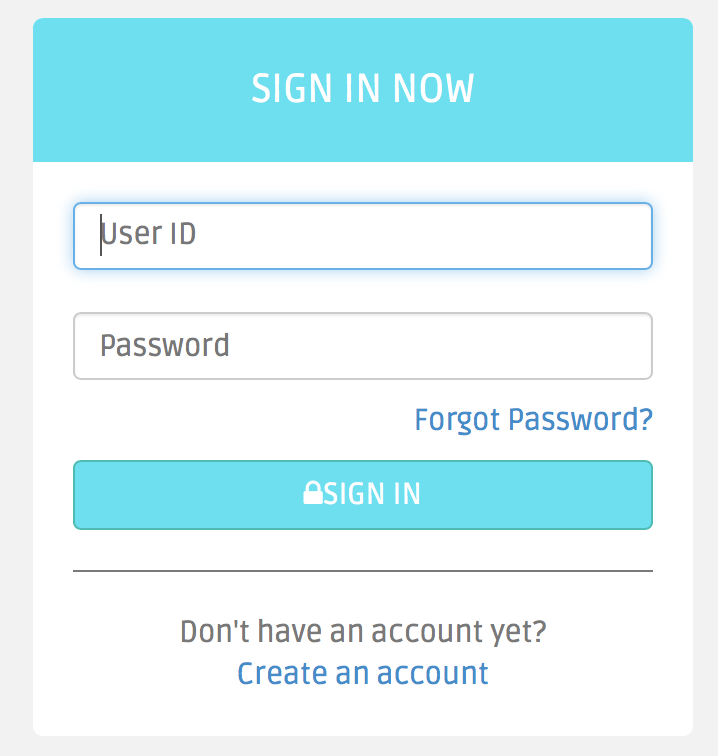
\includegraphics[width=0.4\textwidth]{design/login.png}
  %\hspace{0.5cm}
  %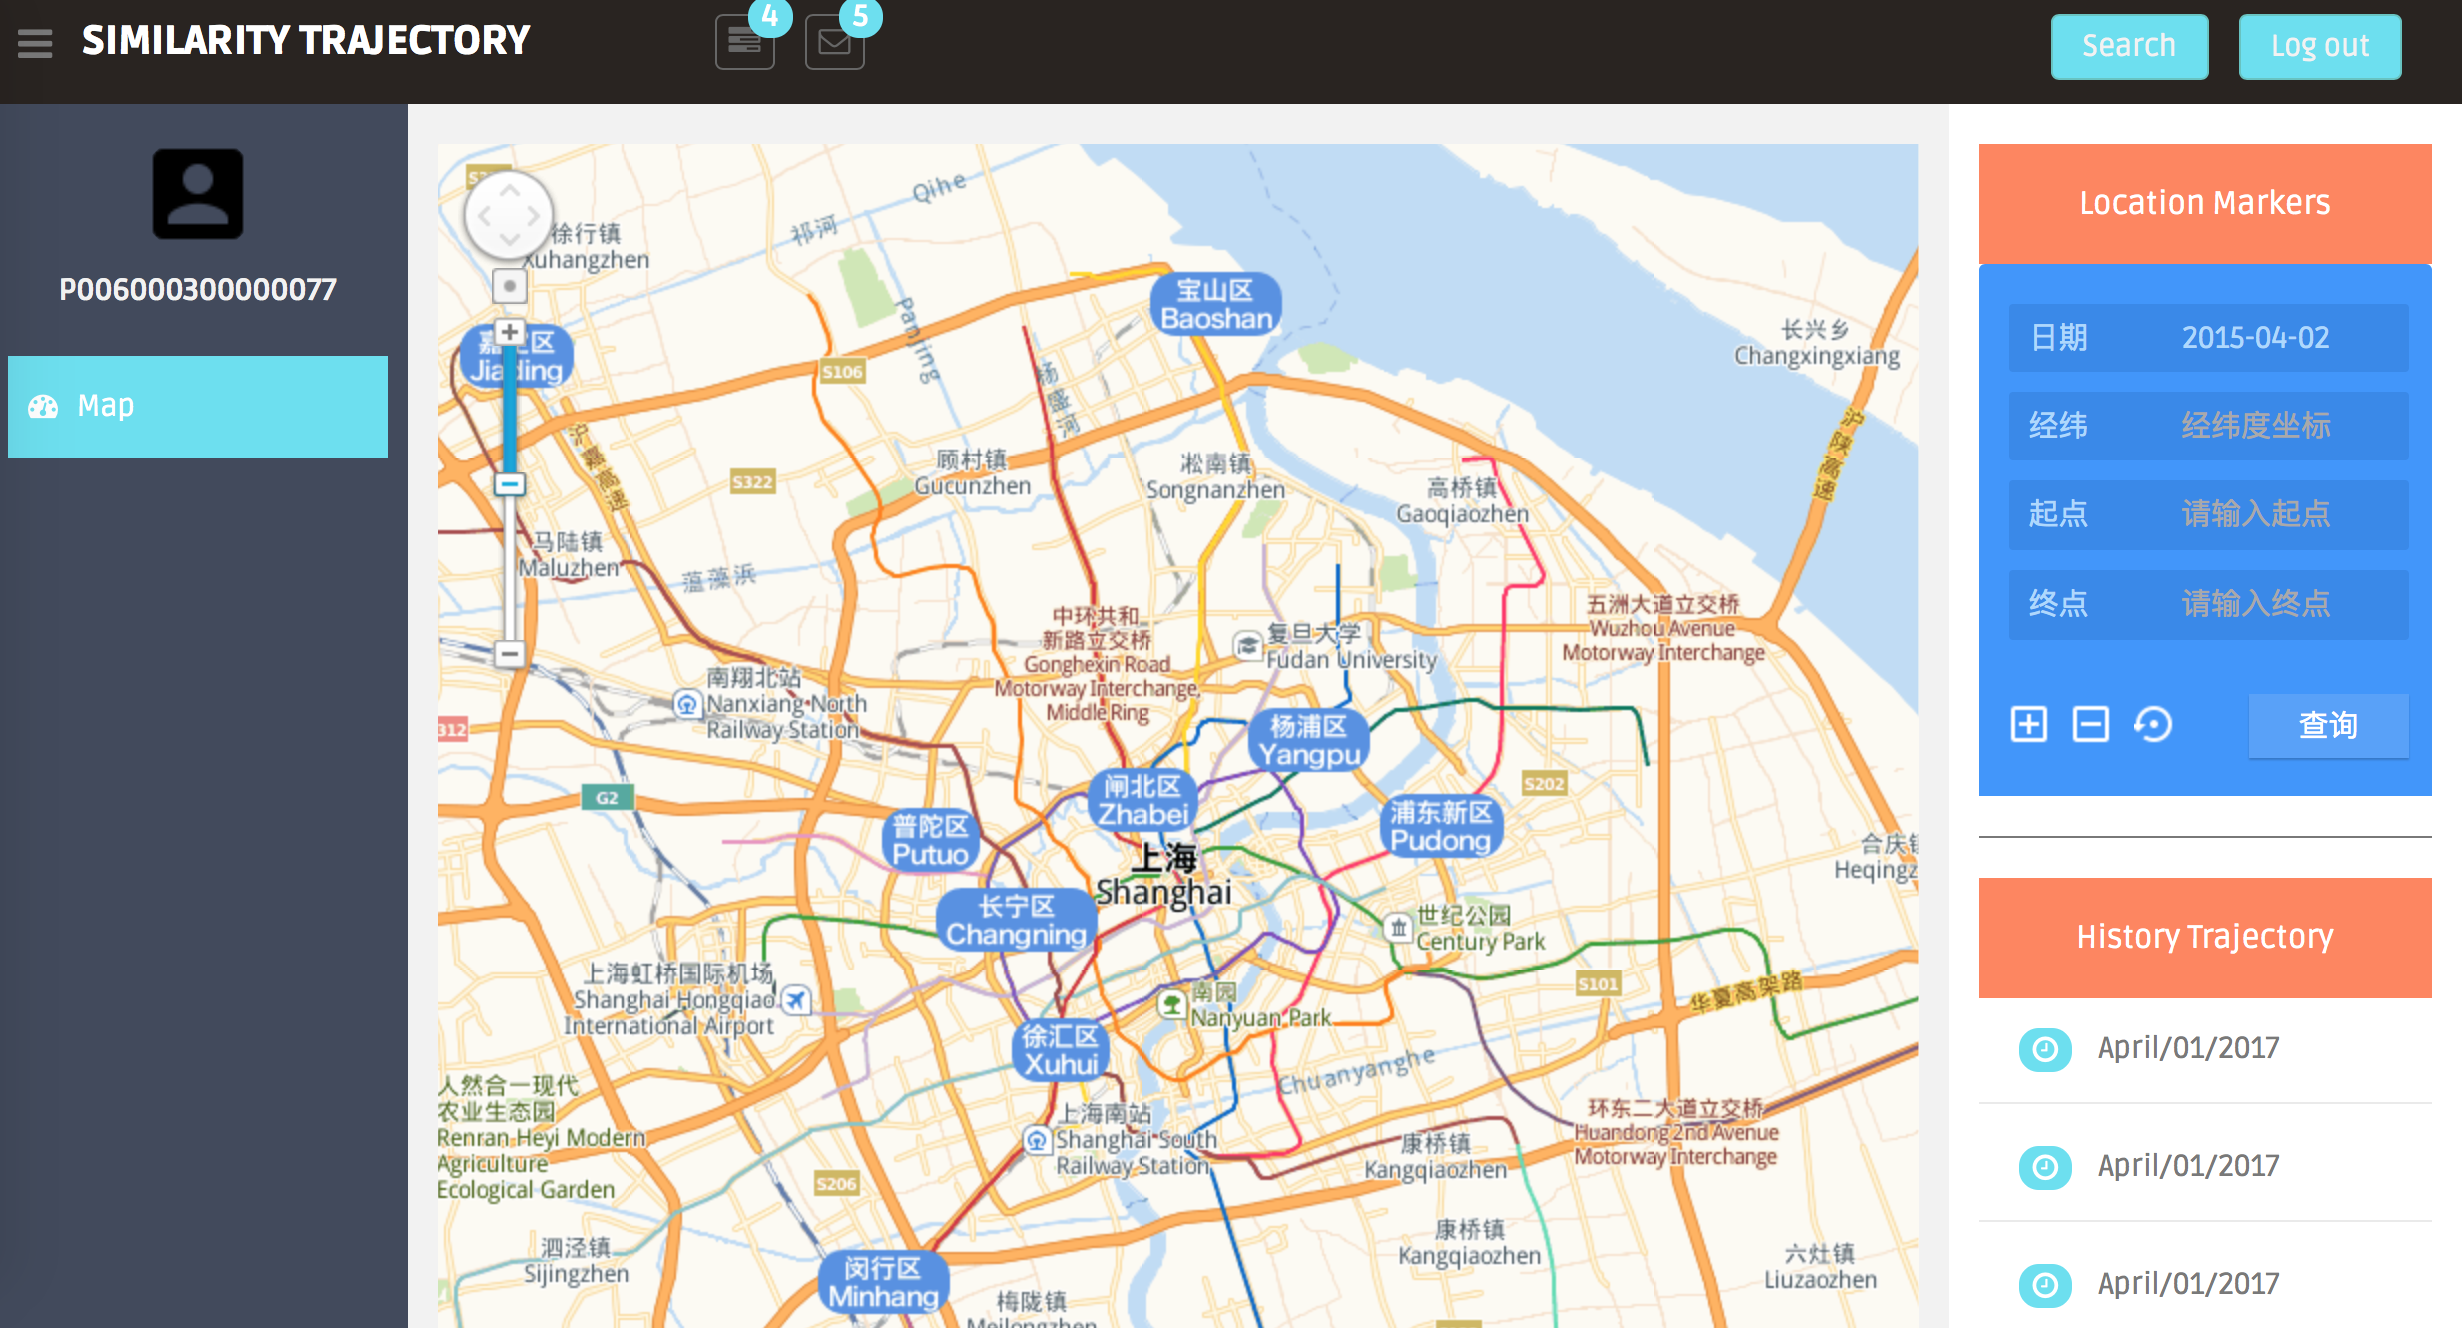
\includegraphics[width=0.6\textwidth]{design/interface.png}
%  \bicaption[fig:login-interface]{用户登录界面}{用户登录界面}{Fig}{User login interface design}
%\end{figure}


\section{系统用户界面设计}
\label{sec:window interface}

图\ref{fig:user-interface}和图\ref{fig:map-interface}分别为用户使用功能的窗口和用户使用系统功能的主要界面设计实现截图。

\begin{figure}[!htp]
	\centering
	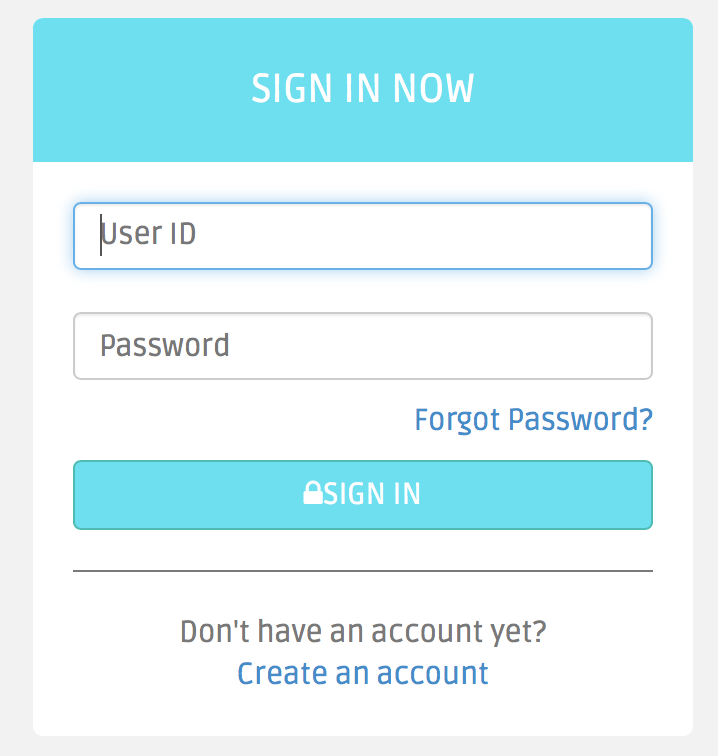
\includegraphics[width=0.3\textwidth]{design/login.png}
	\hspace{0.3cm}
	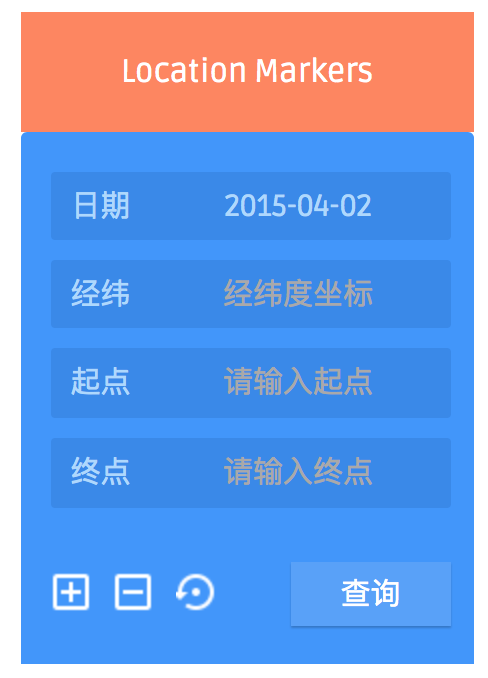
\includegraphics[width=0.3\textwidth]{design/search.png}
   	\hspace{0.3cm}
   	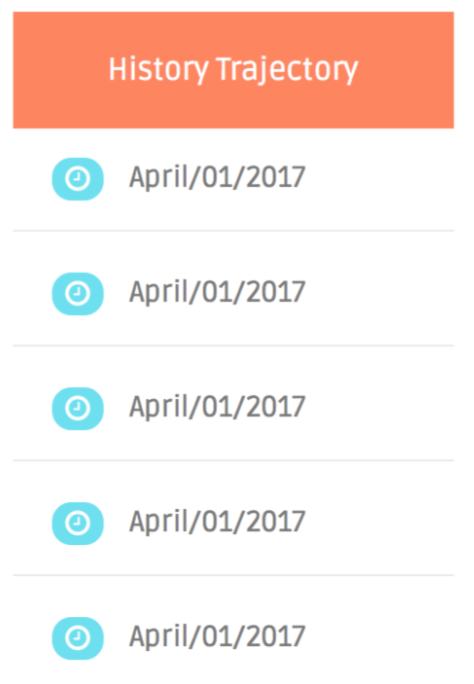
\includegraphics[width=0.3\textwidth]{design/history-trajectory.png}
   	\bicaption[fig:user-interface]{用户功能窗口}{用户功能窗口}{Fig}{User function window interface}
\end{figure}

\begin{figure}[!htp]
  \centering
  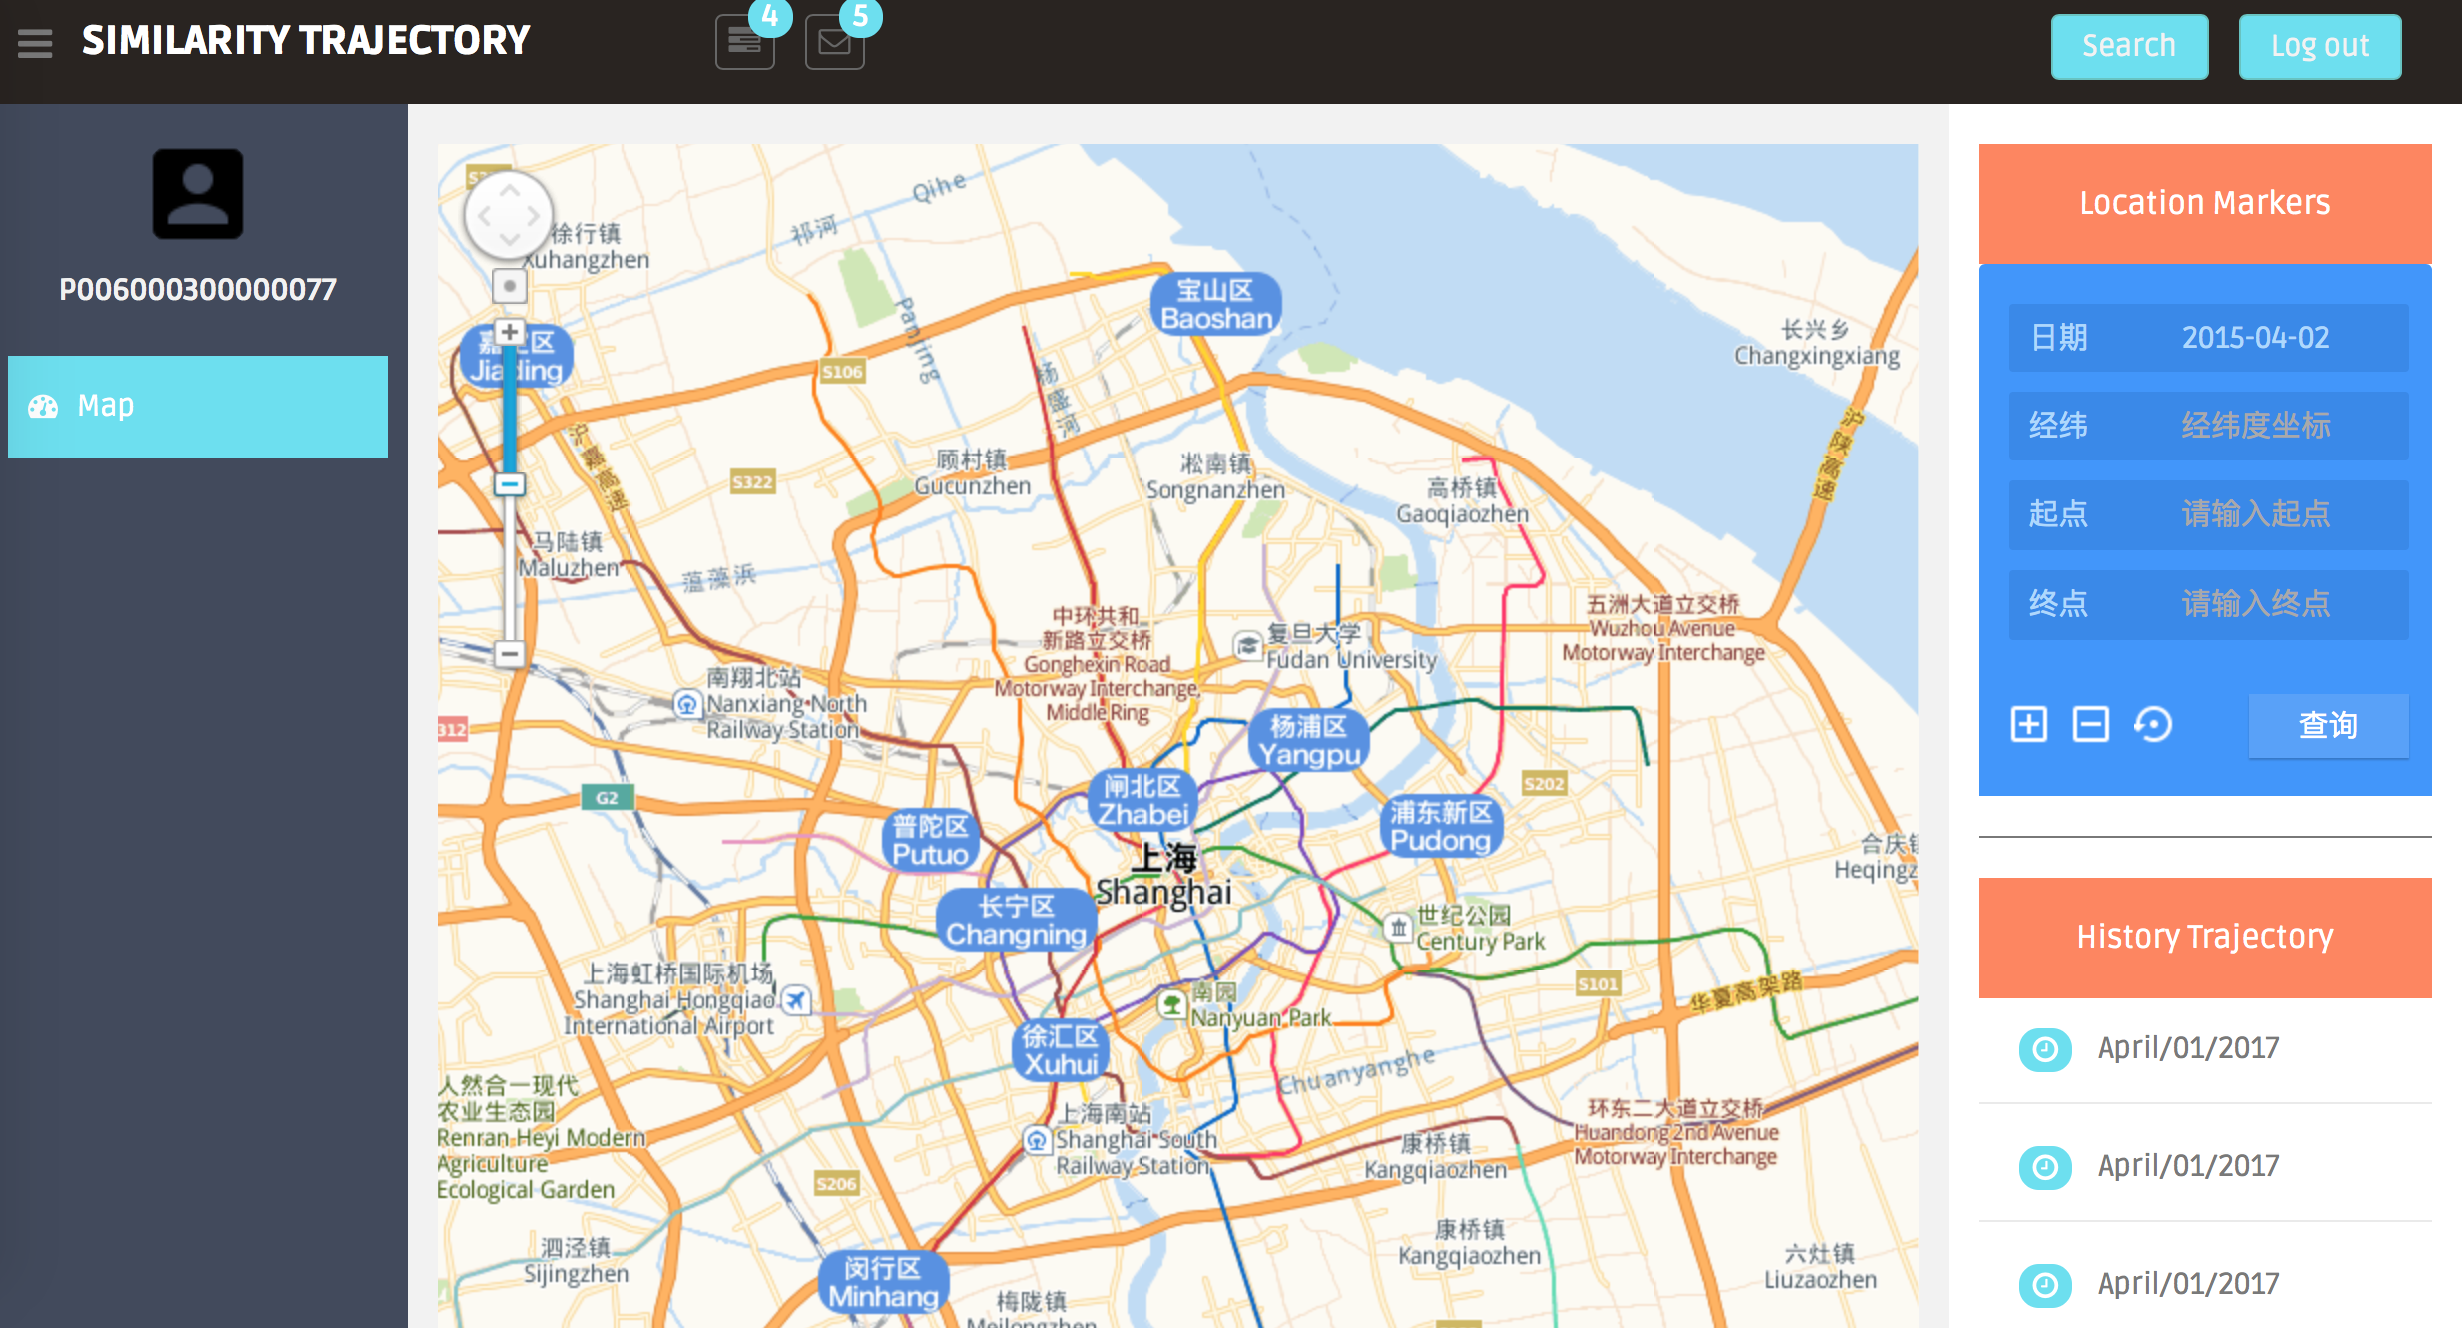
\includegraphics[width=0.7\textwidth]{design/interface.png}
  \bicaption[fig:map-interface]{用户地图界面设计}{用户地图界面设计}{Fig}{User interface design}
\end{figure}

%\begin{figure}[!htp]
%  \centering
%  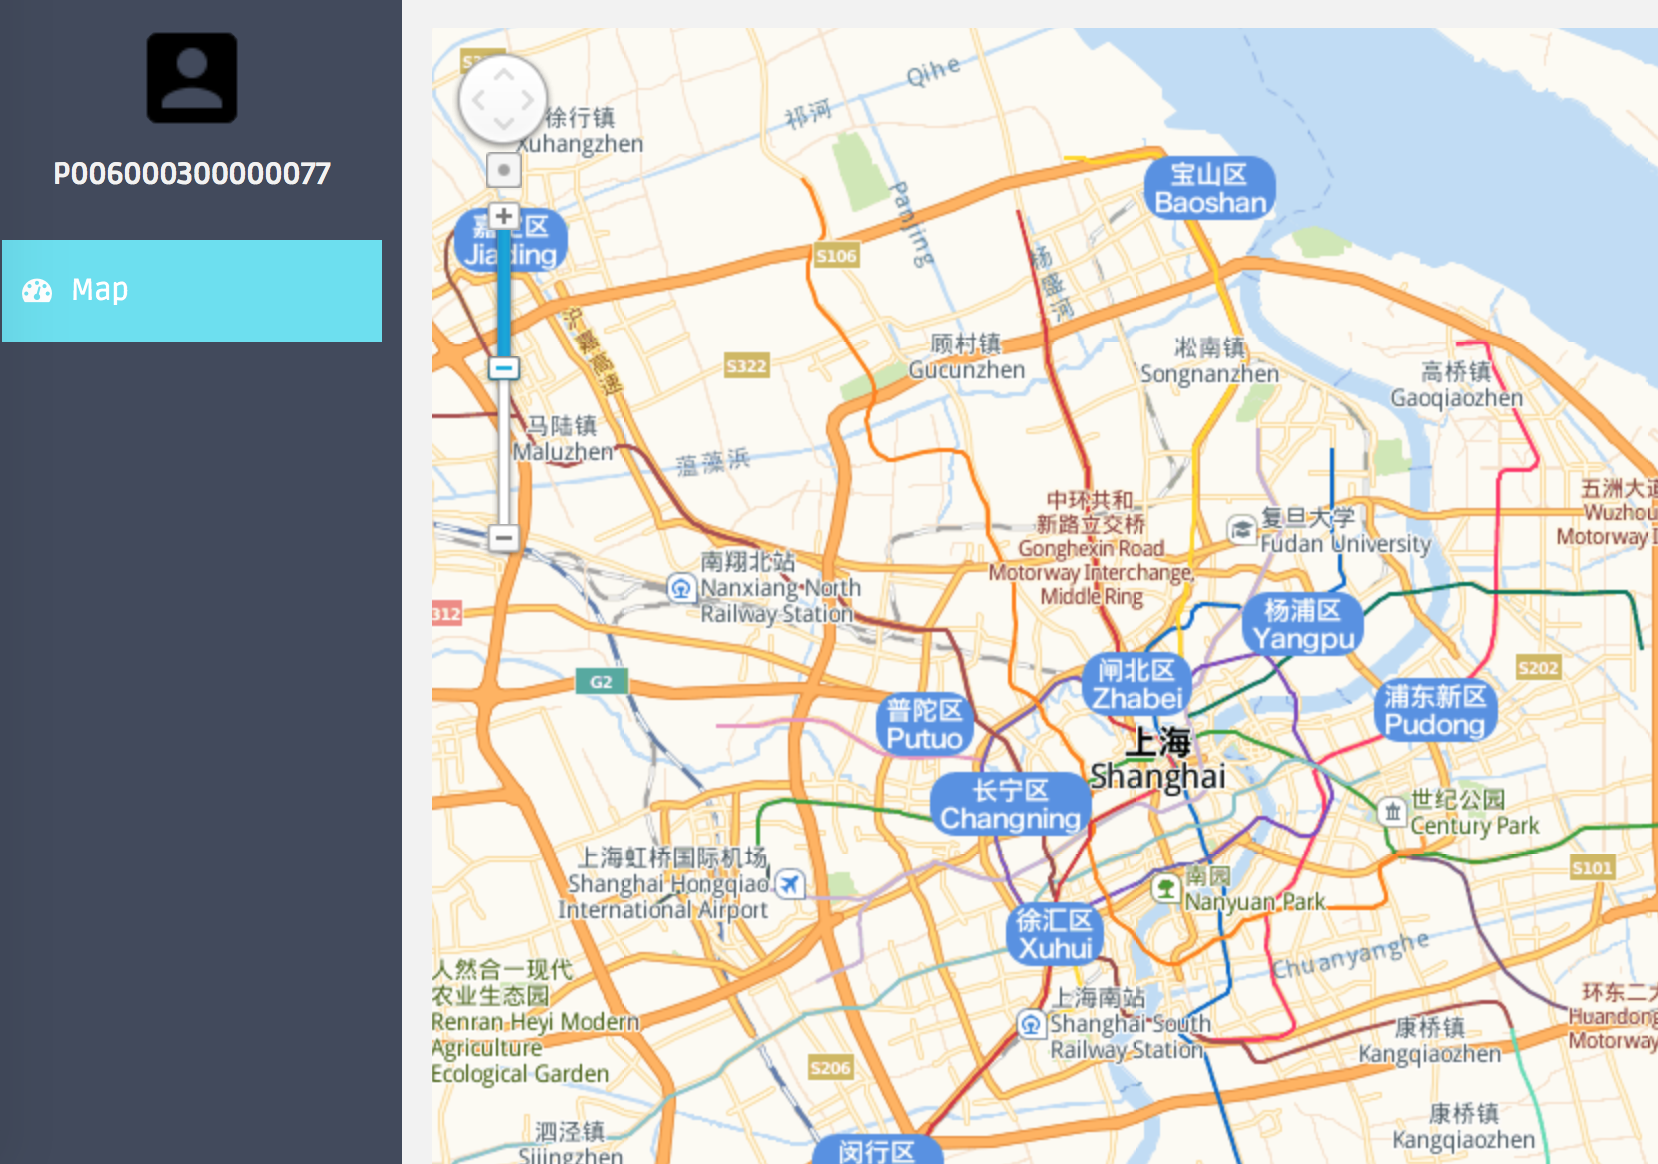
\includegraphics[width=0.4\textwidth]{design/map.png}
%  \bicaption[fig:function-interface]{用户地图界面设计}{用户地图界面设计}{Fig}{User map function interface design}
%\end{figure}


%\subsection{系统性能分析}
%\label{subsec:performance analysis}
%(系统运行截图和系统性能表格)

\section{本章小结}
\label{sec:design conclusion}
本章基于系统需求分析,将上一章节中对系统的需求描述展转换成具体接口设计结构与对应模块设计结构:将一个复杂的相似轨迹查询系统以小模块子系统的结构进行分解,并建立模块之间的数据传递和功能调用关系,确定对应接口对应的数据传递层。在这里,对相似轨迹查询系统进行设计阐述的主要目的是将需求逻辑转化为功能模块实现,以便开发人员在开发这一系统时能清晰明了明确自己负责的模块开发部分,也便于用于理解系统的运行逻辑情况。
